\documentclass[12pt]{article}
\usepackage[left=1cm, right=1cm, top=2cm,bottom=1.5cm]{geometry} 

\usepackage[parfill]{parskip}
\usepackage[utf8]{inputenc}
\usepackage[T2A]{fontenc}
\usepackage[russian]{babel}
\usepackage{enumitem}
\usepackage[normalem]{ulem}
\usepackage{amsfonts, amsmath, amsthm, amssymb, mathtools}

\usepackage{tabularx}
\usepackage{hhline}

\usepackage{accents}
\usepackage{fancyhdr}
\pagestyle{fancy}
\renewcommand{\headrulewidth}{1.5pt}
\renewcommand{\footrulewidth}{1pt}

\usepackage{graphicx}
\usepackage[figurename=Рис.]{caption}
\usepackage{subcaption}
\usepackage{float}

%%Наименование папки откуда забирать изображения
\graphicspath{ {./images/} }

%%Изменение формата для ввода доказательства
\renewcommand{\proofname}{$\square$  \nopunct}
\renewcommand\qedsymbol{$\blacksquare$}

%%Изменение отступа на таблицах
\addto\captionsrussian{%
	\renewcommand{\proofname}{$\square$ \nopunct}%
}
%% Римские цифры
\newcommand{\RN}[1]{%
	\textup{\uppercase\expandafter{\romannumeral#1}}%
}

%% Для удобства записи
\newcommand{\MR}{\mathbb{R}}
\newcommand{\MC}{\mathbb{C}}
\newcommand{\MQ}{\mathbb{Q}}
\newcommand{\MN}{\mathbb{N}}
\newcommand{\MZ}{\mathbb{Z}}
\newcommand{\MTB}{\mathbb{T}}
\newcommand{\MTI}{\mathbb{I}}
\newcommand{\MI}{\mathrm{I}}
\newcommand{\MCI}{\mathcal{I}}
\newcommand{\MJ}{\mathrm{J}}
\newcommand{\MH}{\mathrm{H}}
\newcommand{\MT}{\mathrm{T}}
\newcommand{\MU}{\mathcal{U}}
\newcommand{\MV}{\mathcal{V}}
\newcommand{\MB}{\mathcal{B}}
\newcommand{\MF}{\mathcal{F}}
\newcommand{\MW}{\mathcal{W}}
\newcommand{\ML}{\mathcal{L}}
\newcommand{\MP}{\mathcal{P}}
\newcommand{\VN}{\varnothing}
\newcommand{\VE}{\varepsilon}

\theoremstyle{definition}
\newtheorem{defn}{Опр:}
\newtheorem{rem}{Rm:}
\newtheorem{prop}{Утв.}
\newtheorem{exrc}{Упр.}
\newtheorem{lemma}{Лемма}
\newtheorem{theorem}{Теорема}
\newtheorem{corollary}{Следствие}

\newenvironment{cusdefn}[1]
{\renewcommand\thedefn{#1}\defn}
{\enddefn}

\DeclareRobustCommand{\divby}{%
	\mathrel{\text{\vbox{\baselineskip.65ex\lineskiplimit0pt\hbox{.}\hbox{.}\hbox{.}}}}%
}
%Короткий минус
\DeclareMathSymbol{\SMN}{\mathbin}{AMSa}{"39}
%Длинная шапка
\newcommand{\overbar}[1]{\mkern 1.5mu\overline{\mkern-1.5mu#1\mkern-1.5mu}\mkern 1.5mu}
%Функция знака
\DeclareMathOperator{\sgn}{sgn}

%Функция ранга
\DeclareMathOperator{\rk}{\text{rk}}

%Обозначение константы
\DeclareMathOperator{\const}{\text{const}}

\DeclareMathOperator{\codim}{\text{codim}}

\DeclareMathOperator*{\dsum}{\displaystyle\sum}
\newcommand{\ddsum}[2]{\displaystyle\sum\limits_{#1}^{#2}}

%Интеграл в большом формате
\DeclareMathOperator{\dint}{\displaystyle\int}
\newcommand{\ddint}[2]{\displaystyle\int\limits_{#1}^{#2}}
\newcommand{\ssum}[1]{\displaystyle \sum\limits_{n=1}^{\infty}{#1}_n}

\newcommand{\smallerrel}[1]{\mathrel{\mathpalette\smallerrelaux{#1}}}
\newcommand{\smallerrelaux}[2]{\raisebox{.1ex}{\scalebox{.75}{$#1#2$}}}

\newcommand{\smallin}{\smallerrel{\in}}
\newcommand{\smallnotin}{\smallerrel{\notin}}

\newcommand*{\medcap}{\mathbin{\scalebox{1.25}{\ensuremath{\cap}}}}%
\newcommand*{\medcup}{\mathbin{\scalebox{1.25}{\ensuremath{\cup}}}}%

\makeatletter
\newcommand{\vast}{\bBigg@{3.5}}
\newcommand{\Vast}{\bBigg@{5}}
\makeatother

%Промежуточное значение для sup\inf, поскольку они имеют разную высоту
\newcommand{\newsup}{\mathop{\smash{\mathrm{sup}}}}
\newcommand{\newinf}{\mathop{\mathrm{inf}\vphantom{\mathrm{sup}}}}

%Скалярное произведение
\newcommand{\inner}[2]{\left\langle #1, #2 \right\rangle }
\newcommand{\linsp}[1]{\left\langle #1 \right\rangle }
\newcommand{\linmer}[2]{\left\langle #1 \vert #2\right\rangle }

%Подпись символов снизу
\newcommand{\ubar}[1]{\underaccent{\bar}{#1}}

%% Шапка для букв сверху
\newcommand{\wte}[1]{\widetilde{#1}}
\newcommand{\wht}[1]{\widehat{#1}}

%%Трансформация Фурье
\newcommand{\fourt}[1]{\mathcal{F}\left(#1\right)}
\newcommand{\ifourt}[1]{\mathcal{F}^{-1}\left(#1\right)}

%%Символ вектора
\newcommand{\vecm}[1]{\overrightarrow{#1\,}}

%%Пространстов матриц
\newcommand{\mat}[2]{\operatorname{Mat}_{#1\times #2}}


%%Взятие в скобки, модули и норму
\newcommand{\parfit}[1]{\left( #1 \right)}
\newcommand{\modfit}[1]{\left| #1 \right|}
\newcommand{\sqparfit}[1]{\left\{ #1 \right\}}
\newcommand{\normfit}[1]{\left\| #1 \right\|}

%%Функция для обозначения равномерной сходимости по множеству
\newcommand{\uconv}[1]{\overset{#1}{\rightrightarrows}}
\newcommand{\uconvm}[2]{\overset{#1}{\underset{#2}{\rightrightarrows}}}


%%Функция для обозначения нижнего и верхнего интегралов
\def\upint{\mathchoice%
	{\mkern13mu\overline{\vphantom{\intop}\mkern7mu}\mkern-20mu}%
	{\mkern7mu\overline{\vphantom{\intop}\mkern7mu}\mkern-14mu}%
	{\mkern7mu\overline{\vphantom{\intop}\mkern7mu}\mkern-14mu}%
	{\mkern7mu\overline{\vphantom{\intop}\mkern7mu}\mkern-14mu}%
	\int}
\def\lowint{\mkern3mu\underline{\vphantom{\intop}\mkern7mu}\mkern-10mu\int}

%%След матрицы
\DeclareMathOperator*{\tr}{tr}

\begin{document}
\lhead{Линейная алгебра и геометрия}
\chead{Тимашев Д.А.}
\rhead{Лекция - 4}

\section*{Прямая внешняя сумма}

\begin{theorem}
	Пусть $\dim{V} < \infty$, $U_1, \dotsc, U_m \subseteq V$  - подпространства, тогда следующие условия эквивалентны:
	\begin{enumerate}[label=(\arabic*)]
		\item $U_1,\dotsc, U_m$ - линейно независимы;
		\item Объединение базисов $U_1, \dotsc, U_m$ есть базис $U_1 + \dotsc + U_m$;
		\item $\dim{(U_1 + \dotsc + U_m)} = \dim{U_1} + \dotsc + \dim{U_m}$;
	\end{enumerate}
\end{theorem}

\begin{defn}
	Пусть $V$ - векторное пространство, $U \subseteq V$ - его подпространство, подпространство $W \subseteq V$ такое, что $V = U \oplus W$ называется \uwave{дополнительным} к $U$ подпространством.
\end{defn}

\begin{figure}[H]
	\centering
	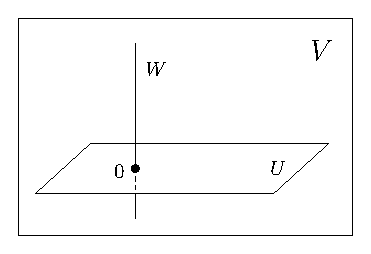
\includegraphics[width=0.24\textwidth]{LAL4_1.eps}
	\caption{Дополнительное к $U$ подпространство $V$.}
	\label{4_1}
\end{figure}

\begin{corollary}
	Если $\dim{V} < \infty \Rightarrow \forall$ подпространства $U \subseteq V, \, \exists\, W \subseteq V \colon V = U \oplus W$.
\end{corollary}
\begin{proof}
	Выберем согласованный с подпространством $U$ базис:
	$$
		(\overbrace{\underbrace{e_1, \dotsc, e_m}_{\text{базис } U}, e_{m+1}, \dotsc, e_n}^{\text{базис }V}), \, U = \linsp{e_1, \dotsc, e_m}, \, V = \linsp{e_1, \dotsc, e_m,e_{m+1}, \dotsc, e_n}
	$$
	Положим, что $W = \linsp{e_{m+1}, \dotsc, e_n} \Rightarrow V = U + W$ по построению, а поскольку объединение базиса $U$ и базиса $W$, равного $(e_{m+1}, \dotsc, e_n)$ по построению, даст нам базис $V$, то по условию $(2)$ теоремы это равносильно линейной независимости подпространств $U$ и $W \Rightarrow$ сумма прямая: $V =U \oplus W$.
\end{proof}

\begin{prop}
	Если $V = U \oplus W \Rightarrow V/U \simeq W$.
\end{prop}
\begin{proof}
	Построим изоморфизм $\varphi \colon W \to V / U$ в явном виде :
	$$
		\forall w \in W, \, \varphi(w) = w + U
	$$
	\textbf{\uline{Инъективность}}: Пусть $\varphi(w) = \varphi(w') \Leftrightarrow w + U = w' + U \Rightarrow \exists \, u \in U \colon w + u = w' = w' + 0$, поскольку у нас прямая сумма, то разложение единственное $\Rightarrow u = 0 \Rightarrow w = w'$.
	
	\textbf{\uline{Сюръективность}}: $\forall v \in V, \, \exists \, u \in U, \, w \in W \colon v = u + w \Rightarrow v + U = w + U \Rightarrow \forall v + U \in V/U, \, \exists \, w \in W$.
	
	Таким образом $\varphi$ - биективное отображение, согласованность с операциями - очевидна:
	$$
		\varphi(\lambda {\cdot} v + \mu{\cdot} w) = (\lambda{\cdot} v + \mu {\cdot}w) + U = \lambda{\cdot} v + U + \mu{\cdot} w + U = \lambda{\cdot}(v + U) + \mu{\cdot}(w + U) = \lambda {\cdot}\varphi(v) + \mu {\cdot}\varphi(w)
	$$
\end{proof}
\begin{rem}
	Заметим, что дополнительное подпространство $W$ не однозначный объект, в то время как фактор-пространство канонически определяется по подпространству и единственным образом.
\end{rem}
\newpage
\section*{Линейный функции}
Изучим функции на векторных пространствах, которые ``уважают'' структуру векторного пространства. Такие функции называются линейными.
\begin{defn}
	Функция $\alpha \colon V \to K$ называется \uwave{линейной}, если верны свойства:
	\begin{enumerate}[label=(\arabic*)]
		\item $\alpha(v + w) = \alpha(v) + \alpha(w), \, \forall v,w \in V$;
		\item $\alpha(\lambda{\cdot}v) = \lambda{\cdot}\alpha(v), \forall v\in V, \, \forall \lambda \in K$;
	\end{enumerate}
\end{defn}

\subsection*{Примеры линейных функций: след матрицы}

\begin{defn}
	$\forall A \in \mat{n}{n}(K), \, \tr{(A)} = a_{11} + a_{22} + \dotsc + a_{nn}$ - \uwave{след матрицы}.
\end{defn}

$V = \mat{n}{n}(K), \, \alpha(A) = \tr{(A)}$, проверим что след является линейной функцией:
\begin{enumerate}[label=(\arabic*)]
	\item $\tr{(A+B)} = (a_{11} + b_{11}) + (a_{22} + b_{22}) + \dotsc + (a_{nn} + b_{nn}) = \tr{(A)} + \tr{(B)} , \, \forall A,B \in V$;
	\item $\tr(\lambda{\cdot}A) = \lambda{\cdot}a_{11} + \dotsc + \lambda{\cdot}a_{nn} = \lambda{\cdot}(a_{11} + \dotsc + a_{nn}) = \lambda{\cdot}\tr{(A)}, \forall A \in V, \, \forall \lambda \in K$;
\end{enumerate}

\subsection*{Примеры линейных функций: линейный функционал}
\begin{defn}
	Функцию на пространстве, которое само состоит из функций называют \uwave{функционалом}.
\end{defn}
$V = \MF(X,K), \, x_0 \in X \Rightarrow \alpha(f) = f(x_0), \, \forall f \in \MF(X,K)$, где $\alpha$ - функционал вычисления значения в фиксированной точке $x_0$. Этот функционал будет линейным функционалом на $\MF(X,K)$:
\begin{enumerate}[label=(\arabic*)]
	\item $\alpha(f + g) = (f+g)(x_0) = f(x_0) + g(x_0) = \alpha(f) + \alpha(g), \, \forall f,g \in V$;
	\item $\alpha(\lambda{\cdot}f) = (\lambda{\cdot}f)(x_0)= \lambda{\cdot}f(x_0) = \lambda{\cdot}f(x_0), \forall f \in V, \, \forall \lambda \in K$;
\end{enumerate}
\hfill\\
Пусть $\dim{V} < \infty$, выберем $(e_1,\dotsc, e_n)$ - базис $V$, хотим понять как вычислить линейную функцию в координатах. Знаем, что: $\forall x \in V, \, \exists!$ разложение $x = x_1 e_1 + \dotsc + x_n e_n$, тогда:
$$
	\forall x \in V, \, \exists! \, X \colon x = eX = x_1 e_1 + x_n e_n \Rightarrow
$$
$$
	\Rightarrow \alpha(x) = \alpha(x_1 e_1) + \dotsc + \alpha(x_n e_n) = x_1{\cdot}\alpha(e_1) + \dotsc + x_n{\cdot}\alpha(e_n)
$$
Если обозначить коэффициенты $\alpha(e_i) = a_i, \, \forall i = \overline{1,n}$, то получим следующее выражение:
$$
	\forall x \in V, \, \alpha(x) = a_1{\cdot}x_1 + \dotsc + a_n{\cdot}x_n
$$
Любая линейная функция в координатах записывается как линейная комбинация координат вектора с какими-то фиксированными коэффициентами - значениями на базисных векторах.
\begin{defn}
	Линейная комбинация переменных с фиксированными коэффициентами, то есть однородный многочлен первой степени от координат, называется \uwave{линейной формой}.
\end{defn}
\begin{rem}
	Обратно тоже верно, каждая линейная форма задает линейную функцию (по равенству выше):
	$$
		\alpha(\lambda x + \mu y) = (\lambda x_1 + \mu y_1){\cdot}a_1 + \dotsc (\lambda x_n + \mu y_n){\cdot}a_n = \lambda x_1 {\cdot}a_1 + \mu y_1{\cdot}a_1 + \dotsc + \lambda x_n {\cdot}a_n + \mu y_n{\cdot}a_n = 
	$$
	$$	
		= \lambda(x_1 {\cdot}a_1 + \dotsc + x_n{\cdot} a_n) + \mu(y_1{\cdot} a_1 + \dotsc + y_n {\cdot}a_n) = \lambda\alpha(x) + \mu\alpha(y)
	$$
\end{rem}
Другими словами, линейная форма это способ записи линейных функций в координатах, если мы зафиксировали базис. В другом базисе та же самая функция будет задаваться какой-то другой линейной формой, можно написать как переход от одной к другой, поскольку мы знаем как меняется базис.

\subsection*{Сопряженное пространство}
\begin{prop}
	Множество всех линейных функций на $V$ это подпространство $V^* \subseteq \MF(V,K)$ пространства всех функций на $V$. 
\end{prop}
\begin{defn}
	Подпространство $V^* \subseteq \MF(V,K)$ всех линейных функций на $V$ называется \uwave{сопряженным} или \uwave{двойственным}, или \uwave{дуальным} пространством к $V$. Базис этого пространства называется \uwave{сопряженным} или \uwave{двойственным}, или \uwave{дуальным} базисом к базису пространства $V$.
\end{defn}
\begin{proof}
	Докажем, что $V^*$ это подпространство.
	\begin{enumerate}[label=\arabic*)]
		\setcounter{enumi}{-1}
		\item \textbf{\uline{Непустота}}: $\alpha(x) \equiv 0 \in V^{*}$, поскольку для нулевой функции очевидно выполняются свойства линейности;
		$$
			0(\lambda v + \mu w) = \alpha{\cdot}0(v) + \mu{\cdot}0(w) = 0 + 0 = 0
		$$
		\item \textbf{\uline{Замкнутость по сложению}}: $\forall \alpha, \beta \in V^* \Rightarrow \alpha + \beta \in V^*$:
		$$
			(\alpha + \beta)(\lambda v + \mu w) = \lambda \alpha(v) + \mu\alpha(w) + \lambda \beta(v) + \mu\beta(w) = \lambda(\alpha + \beta)(v) + \mu(\alpha + \beta)(w)
		$$
		\item \textbf{\uline{Замкнутость по умножению на скаляр}}: $\forall \alpha \in V^*, \, \lambda \in K \Rightarrow \lambda{\cdot}\alpha \in V^*$;
		$$
			(\lambda{\cdot}\alpha)(\mu v + \gamma w) = \lambda{\cdot}\mu{\cdot}\alpha(v) + \lambda{\cdot}\gamma{\cdot}\alpha(w) = \mu{\cdot}(\lambda{\cdot}\alpha)(v) + \gamma{\cdot}(\lambda{\cdot}\alpha)(w)
		$$
	\end{enumerate}
\end{proof}

\begin{prop}
	Если $\dim{V}= n < \infty$, то $\dim{V^*} = n$.
\end{prop}
\begin{proof}
	Выберем в пространстве $V$ произвольный базис $e = (e_1, \dotsc, e_n)$. Тогда мы можем расписать любую линейную функцию в этом базисе, как линейную форму. Рассмотрим \uwave{координатные функции} $\VE_i \in V^*$ на пространстве $V$: 
	$$
		x = x_1e_1 + \dotsc + x_n e_n \in V \Rightarrow \VE_i(x) = x_i, \, \forall i = \overline{1,n}
	$$
	Это простейшая линейная форма, где от каждого вектора просто берется его координата $\Rightarrow$ тоже линейная функция. Докажем, что набор координатных функций $\VE = (\VE_1,\dotsc, \VE_n)$ будет базисом сопряженного пространства: $\VE$ порождает сопряженное пространство и функции $\VE_i$ линейно независимы.
	\begin{enumerate}[label=\arabic*)]
		\item \textbf{\uline{Порождение подпространства}}: Рассмотрим произвольную линейную функцию на $V$:
		$$
			\forall \alpha \in V^*, \, \forall x \in V \colon \alpha(x) = a_1x_1 + \dotsc a_n x_n, \, \alpha(e_i) = a_i, \, \forall i = \overline{1,n}
		$$
		Представление функции выше верно для конкретного вектора $x$, значения функции $\alpha$ на базисных векторах $e_i$ полностью определяют линейную форму $\Rightarrow$ для произвольного вектора $x$:
		$$
			\alpha(x) = a_1\VE_1(x) + \dotsc + a_n\VE_n(x)
		$$
		то есть любая линейная функция $\alpha(x)$ есть линейная комбинация координатных функций с коэффициентами $a_i = \alpha(e_i)$. Следовательно, $V^* = \linsp{\VE_1, \dotsc, \VE_n}$. 
		\item \textbf{\uline{Линейная независимость}}: Пусть верно:
		$$
			\lambda_1 \VE_1 + \dotsc + \lambda_n \VE_n= \lambda_1 \VE_1(x) + \dotsc + \lambda_n \VE_n(x) = 0
		$$
		Подставим в это функциональное равенство какое-нибудь $e_i$:
		$$
			0 =\lambda_1 \VE_1(e_i) + \dotsc + \lambda_i \VE(e_i) + \dotsc + \lambda_n \VE(e_i) = 0 + \dotsc + \lambda_i{\cdot}1 + \dotsc 0 = \lambda_i \Rightarrow \lambda_i = 0, \,  \forall i = \overline{1,n}
		$$
	\end{enumerate}
\end{proof}
\newpage

\begin{corollary}
	Если $V$ - конечномерно ($\dim{V} < \infty$), то $V \simeq V^*$.
\end{corollary}
\begin{proof}
	Сопряженное пространство имеет ту же самую размерность $\Rightarrow$ поскольку все конечномерные векторные пространства одной и той же размерности изоморфны друг другу, то $V \simeq V^*$.
\end{proof}
\begin{rem}
	Заметим, что этот изоморфизм - не является каноническим, то есть он зависит от выбора базиса. Тем не менее, можно построить канонический изоморфизм $V \xrightarrow[]{\sim} (V^*)^*$.
\end{rem}

Рассмотрим $\forall  v \in V$ линейный функционал (функцию на пространстве функций): 
$$
	\wht{v} \colon V^* \to K
$$ 
который определяется по следующему правилу:
$$
	\wht{v}(\alpha) = \alpha(v), \, \forall \alpha \in V^*
$$
Это функционал вычисления значения линейной функции в фиксированной точке $v \Rightarrow$ с каждым вектором пространства $V$ мы связали линейный функционал на сопряженном пространстве $V^*$. 

\begin{theorem}
	Если $\dim{V} < \infty$, то $\exists$ канонический изоморфизм: $V \xrightarrow[]{\sim}(V^*)^*$, то есть не зависящий от выбора базиса в $V$, который сопоставляет каждому вектору из $V$ функционал из $(V^*)^*$: 
	$$
		\psi \colon v \mapsto \wht{v},\, \forall v \in V
	$$
\end{theorem}
\begin{proof}\hfill
	\begin{enumerate}[label=\arabic*)]
		\item Докажем, что отображение $\psi \colon V \to (V^*)^*$ согласовано с операциями $(+)$ и $(\; {\cdot}\; )$:
		$$
			\psi(v+w) = \wht{v + w}(\alpha) = \alpha(v + w) = \alpha(v) + \alpha(w) = \wht{v}(\alpha) + \wht{w}(\alpha) = \psi(v) + \psi(w), \, \forall \alpha \in V^* \Rightarrow
		$$
		$$
			\Rightarrow \psi(v+w) = \wht{v + w} = \wht{v} + \wht{w} = \psi(v) + \psi(w)
		$$
		То есть, линейный функционал на $V^*$, отвечающий сумме двух векторов это сумма линейных функционалов, отвечающих отдельным векторам. Аналогично:
		$$
			\psi(\lambda{\cdot}v) = \wht{\lambda{\cdot}v}(\alpha) = \alpha(\lambda{\cdot} v) = \lambda {\cdot}\alpha(v) = \lambda {\cdot}\wht{v}(\alpha) = \lambda{\cdot}\psi(v) , \, \forall \alpha \in V^*, \, \forall \lambda \in K \Rightarrow 
		$$
		$$	
			\Rightarrow \psi(\lambda{\cdot}v) = \wht{\lambda v} = \lambda{\cdot}\wht{v} = \lambda{\cdot}\psi(v)
		$$
		То есть, линейный функционал, отвечающий $\lambda v$ это функционал, отвечающий вектору $v$, умноженный на $\lambda$. 
		
		\item Возьмем какой-нибудь базис $(e_1,\dotsc,e_n)$ пространства $V$, возьмем сопряженный ему базис $(\VE_1, \dotsc, \VE_n)$ пространства $V^*$, тогда:
		$$
			\forall \alpha \in V^*, \, \alpha = a_1\VE_1 + \dotsc + a_n \VE_n, \, a_i = \alpha(e_i), \, \forall i = \overline{1,n} \Rightarrow
		$$
		$$
			\Rightarrow \psi(e_i) = \wht{e}_i(\alpha) = \alpha(e_i) = a_i, \, \forall \alpha \in V^*
		$$
		Отсюда мы видим, что $\wht{e}_i$ это координатная функция на пространстве $V^*$ по отношению к базису сопряженного пространства $(\VE_1,\dotsc, \VE_n) \Rightarrow$ набор функционалов $\left(\wht{e}_1,\dotsc, \wht{e}_n\right)$ - это базис второго сопряженного пространства $(V^*)^*$, сопряженного к первому сопряженному $V^*$.
		
		\item Докажем биективность отображения. $\forall x \in V, \, x = x_1 e_1 + \dotsc x_n e_n \Rightarrow$ по пункту $1)$ функционал $\wht{x}$, соответствующий этому вектору, будет иметь вид:
		$$
			\wht{x} = x_1{\cdot}\wht{e}_1 + \dotsc + x_n{\cdot}\wht{e}_n
		$$
		Таким образом, у $x$ и $\wht{x}$ одинаковый набор координат в соответствующих базисах $\Rightarrow$ это взаимооднозначное соответствие, поскольку вектор однозначно определяется и однозначно определяет набор своих координат.
	\end{enumerate}
\end{proof}

\subsection*{Двойственность (конечномерный случай)}
Элементы $V$ называем \uwave{векторами}, элементы сопряженного пространства $V^*$, то есть линейные функции на пространстве $V$, принято называть \uwave{ковекторами}. В силу канонического изоморфизма, векторы можно отождествить с элементами пространства $(V^*)^*$, то есть линейными функциями на ковекторах.
\begin{defn}
	\uwave{Ковекторами} будем называть линейные функции на векторах.
\end{defn}
\begin{defn}
	\uwave{Векторами} будем называть линейные функции на ковекторах.
\end{defn}

\begin{defn}
	\uwave{Спаривание} ковектора $\alpha$ с вектором $x$ это значение ковектора на этом векторе или значение на ковекторе $\alpha$ линейного функционала, соответствующего вектору $x$:
	$$
		\linmer{\alpha}{x} \coloneqq \alpha(x) = \wht{x}(\alpha)
	$$
	\textbf{\uline{Обозначение}}: $\linmer{\alpha}{x}$.
\end{defn}
Спаривание можно расписать в координатах:
$$
	\linmer{\alpha}{x} = \alpha(x) = a_1 x_1 + \dotsc + a_n x_n, \quad a_i = \linmer{\alpha}{e_i} = \alpha(e_i), \, x_i = \linmer{\VE_i}{x} = \VE_i(x), \, \forall i = \overline{1,n}
$$
\begin{defn}
	\uwave{Условие сопряженности базисов в пространствах} $V$ и $V^*$: базис $(e_1,\dotsc, e_n)$ пространства $V$ сопряжен базису $(\VE_1, \dotsc, \VE_n)$ пространства $V^*$, если выполняется равенство:
	$$
		\linmer{\VE_i}{e_j} = \delta_{ij} = \left\{
		\begin{array}{rl}
			1, & i = j\\
			0, & i \neq j
		\end{array}
		\right.
	$$
	то есть мы хотим сказать, что $\VE_i$ это координатные функции в базисе из $e_j$.
\end{defn}
\begin{rem}
	Любой базис $V^*$ сопряжен некоторому базису $V$, потому что у базиса в $V^*$ существует свой сопряженный базис в $(V^*)^* = V^{**} \simeq V \Rightarrow$ можно считать, что этот сопряженный базис находится в $V$ и удовлетворяет условию сопряженности:
	$$
		\linmer{\VE_i}{e_j} = \wht{e}_j(\VE_i) = \VE_i(e_j) = \delta_{ij}
	$$
\end{rem}

\textbf{Разложение векторов и ковекторов по базисам}:
$$
	\forall x \in V, \, x = x_1 e_1 + \dotsc + x_n e_n = \ddsum{i = 1}{n}\linmer{\VE_i}{x}{\cdot}e_i
$$
$$
	\forall \alpha \in V^*, \, \alpha = a_1 \VE_1 + \dotsc + a_n \VE_n = \ddsum{ i = 1}{n}\linmer{\alpha}{e_i}{\cdot}\VE_i
$$
\newpage
\section*{Линейные функции и подпространства}
\begin{defn}
	Пусть $S \subseteq V$ - произвольное множество векторов в пространстве $V$. Назовём \uwave{аннулятором множества} $S$ множество ковекторов, которые на множестве $S$ обращаются в ноль:
	$$
		S^{\circ} = \{\alpha \in V^* \mid \linmer{\alpha}{v} = 0, \, \forall v \in S\}
	$$
\end{defn}
\begin{prop}(\textbf{Свойства аннуляторов}):
	\begin{enumerate}[label=\arabic*)]
		\item $S^{\circ} \subseteq V^*$ - подпространство;
		\item Если $S \subseteq \wte{S} \Rightarrow S^{\circ} \supseteq \wte{S}^{\circ}$;
		\item $S^{\circ} = \linsp{S}^{\circ}$;
		\item Пусть $T = \linsp{\alpha_1,\dotsc, \alpha_m} \subseteq V^*$, тогда $T^{\circ} \subseteq V^{**} \simeq V$; 
	\end{enumerate}
\end{prop}
\begin{proof}\hfill
	\begin{enumerate}[label=\arabic*)]
		\item Нужно убедиться, что аннулятор замкнут относительно сложения и умножения на скаляры:
		$$
			\forall \alpha,\beta \in S^{\circ}, \, \forall \mu, \lambda \in K, \, \linmer{\mu{\cdot} \alpha + \lambda{\cdot}  \beta}{v} = (\mu{\cdot}\alpha + \lambda{\cdot} \beta)(v) = \mu{\cdot} \alpha(v) + \lambda{\cdot} \beta(v) = 0
		$$
		И нулевая функция также, очевидно, принадлежит $S^{\circ}$;
		\item $S \subseteq \wte{S} \Rightarrow \forall \alpha \in \wte{S}^{\circ}, \, \linmer{\alpha}{v} = 0, \, \forall v \in \wte{S} \Rightarrow \linmer{\alpha}{v} = 0, \, \forall v \in S \Rightarrow \alpha \in S^{\circ} \Rightarrow \wte{S}^{\circ} \subseteq S^{\circ}$; 
		
		\item Проверим в явном виде:
		$$
			\forall \alpha \in S^{\circ}, \, \forall v \in S, \, \linmer{\alpha}{v} = 0 \Rightarrow \forall v_1, \dotsc, v_n \in S, \, \forall \mu_1,\dotsc,\mu_n, \, \linmer{\alpha}{\mu_1 v_1 + \dotsc + \mu_n v_n} = 
		$$
		$$
			= \alpha(\mu_1 v_1 + \dotsc + \mu_n v_n) = \mu_1 \alpha(v_1) + \dotsc + \mu_n\alpha(v_n) = 0 + \dotsc + 0 = 0 \Rightarrow S^{\circ} \subseteq \linsp{S}^{\circ}
		$$
		В обратную сторону очевидно, поскольку $S \subseteq \linsp{S} \Rightarrow S^{\circ} \supseteq \linsp{S}^{\circ}$;
		
		\item По определению и в силу изоморфизма, мы получим:
		$$
			T^{\circ} = \left\{ \wht{x} \in V^{**} \mid \forall i = \overline{1,m}, \, \linmer{\alpha_i}{x} = \wht{x}(\alpha_i) = 0 \right\} = \left\{x \in V \mid \forall i =\overline{1,m}, \, \linmer{\alpha_i}{x} = 0\right\}
		$$
		Если выбрать в $V$ какой-то базис, записать ковекторы в виде линейных форм в этом базисе и записать это выражение в координатах, то мы получим следующее:
		$$
			\alpha_i = a_{i1}\VE_1 + \dotsc + a_{in}\VE_n \Rightarrow \linmer{\alpha_i}{x} = \alpha_i(x) = a_{i1} x_1 + \dotsc a_{in} x_n = 0
		$$
		то есть, аннулятор подпространства $T$ это пространство решений однородной СЛУ;
	\end{enumerate}
\end{proof}
\begin{rem}
	Свойство $3)$ сводит нас к изучению аннуляторов подпространств, если нас интересует, как устроены аннуляторы тех или иных множеств векторов.
\end{rem}

\newpage
\begin{theorem}(\textbf{основная теорема про аннулятор})
	Пусть $V$ - конечномерно и $U\subseteq V$ - подпространство, тогда верны следующие свойства:
	\begin{enumerate}[label=\arabic*)]
		\item $\dim{U^{\circ}} = \codim{U} = \dim{V} - \dim{U}$;
		\item $(U^{\circ})^{\circ} = U$;
	\end{enumerate}
\end{theorem}
\begin{proof}
	Выберем согласованный базис $(e_1,\dotsc, e_m, e_{m+1}, \dotsc, e_n)$ так, чтобы:
	$$
		U = \linsp{e_1,\dotsc, e_m}, \, V = \linsp{e_1,\dotsc, e_m, e_{m+1}, \dotsc, e_n}
	$$
	Пусть $(\VE_1,\dotsc,\VE_n)$ - сопряженный базис в $V^*$. Тогда, поскольку $U = \linsp{e_1,\dotsc, e_m}$, то по определению:
	$$
		\alpha = a_1 \VE_1 + \dotsc + a_n \VE_n \in U^{\circ} \Leftrightarrow \forall i = \overline{1,m}, \, \linmer{\alpha}{e_i} = a_i = 0
	$$
	Следовательно, $U^{\circ} = \linsp{\VE_{m+1}, \dotsc, \VE_n}$.
	\begin{enumerate}[label=\arabic*)]
		\item $\dim{U^{\circ}} = \dim{V} - \dim{U} = n - m = \codim{U}$;
		\item По определению аннулятора $U$:
		$$
			\forall x \in U, \, \forall \alpha \in U^{\circ}, \, \linmer{\alpha}{x} = 0 \Rightarrow x \in (U^{\circ})^{\circ} \Rightarrow U \subseteq (U^{\circ})^{\circ}
		$$
		По пункту $1)$ будет верно: 
		$$
			\dim{U^{\circ\circ}} = \dim{V^*} - \dim{U^{\circ}} = \dim{V^*} - \dim{V} + \dim{U} = \dim{U}
		$$ 
		Тогда по утверждению $3$ лекции $2$ подпространства $U$ и $U^{\circ\circ}$ - совпадают.
	\end{enumerate}
\end{proof}

\subsection*{Задание подпространства с помощью ОСЛУ}

Пусть $U = \linsp{v_1, \dotsc,v_m}$, где векторы не обязаны быть базисом. Тогда $U^{\circ}$ задаёт ОСЛУ вида:
$$
	\left\{
	\begin{array}{ccccc}
		\linmer{\alpha}{v_1} & = & a_1 v_{11} + \dotsc + a_n v_{n1}  & = & 0 \\
		\vdots & \vdots & \vdots & \vdots & \vdots\\
		\linmer{\alpha}{v_m} & = & a_1 v_{m1} + \dotsc + a_n v_{mn} & = & 0
	\end{array}
	\right.
$$
Аннулятор состоит из тех $\alpha$ для которых выполнены уравнения выше, то есть ОСЛУ на коэффициенты линейной функции $a_i$. Если какое-то подпространство задано с помощью ОСЛУ, то мы можем найти его базис (процедура нахождения ФСР для ОСЛУ), тогда $U^{\circ} = \linsp{\alpha_1,\dotsc,\alpha_k}$. В этом случае аннулятор аннулятора, который канонически отождествляется с $U$ по теореме $3$ выше, то есть $U = U^{\circ\circ}$, по аналогии выше задается ОСЛУ:
$$
	\left\{
	\begin{array}{ccccc}
		\linmer{\alpha_1}{x} & = & a_{11} x_{1} + \dotsc + a_{1n} x_{n}  & = & 0 \\
		\vdots & \vdots & \vdots & \vdots & \vdots\\
		\linmer{\alpha_k}{x} & = & a_{k1} x_{1} + \dotsc + a_{kn} x_{n} & = & 0
	\end{array}
	\right.
$$
то есть, это подпространство состоит из тех векторов на которых все ковекторы $\linsp{\alpha_1,\dotsc,\alpha_k}$ обращаются в ноль, что и задается системой выше.

\textbf{\uline{Итог}}: система порождающих для подпространства даёт нам линейные уравнения для аннулятора, а система порождающих для аннулятора даёт нам линейные уравнения для подпространства. То есть при переходе к аннулятору, система порождающих и система линейных уравнений меняются ролями. А поскольку мы умеем искать базис пространства, заданного СЛУ, то мы можем перейти от задания подпространства как линейной оболочки к заданию подпространства СЛУ. Обратный переход мы умели делать и раньше (нахождение ФСР).

\begin{corollary}
	Пусть $\dim{V} = n < \infty$. Набор линейных функций $(\alpha_1,\dotsc,\alpha_n)$ является базисом $V^*$ тогда и только тогда, когда ОСЛУ:
	$$
		\left\{
		\begin{array}{ccccc}
			\linmer{\alpha_1}{x} & = & a_{11} x_{1} + \dotsc + a_{1n} x_{n}  & = & 0 \\
			\vdots & \vdots & \vdots & \vdots & \vdots\\
			\linmer{\alpha_n}{x} & = & a_{n1} x_{1} + \dotsc + a_{nn} x_{n} & = & 0
		\end{array}
		\right.
	$$
	имеет единственное решение $x = 0$.
\end{corollary}
\begin{proof}
	Надо доказать, что существует один единственный вектор, на котором все эти линейные функции обращаются в ноль. $(\alpha_1,\dotsc,\alpha_n)$ - базис $V^* \Leftrightarrow \linsp{\alpha_1,\dotsc,\alpha_n} = V^*$. Если эти ковекторы порождают $V^*$, но линейно зависимы, тогда из них можно было бы убрать лишние и получить базис из меньше чем $n$ ковекторов, но $\dim{V^*} = n$. Очевидно, что:
	$$
		\linsp{\alpha_1,\dotsc,\alpha_n} = V^* \Leftrightarrow \linsp{\alpha_1,\dotsc,\alpha_n}^{\circ} = (V^*)^{\circ}
	$$
	Множество $(V^*)^{\circ}$ это множество тех векторов, на которых все линейные функции обращаются в ноль, но такой вектор только один - $\{0\}$. Если вектор не $\{0\}$, то у него есть хоть какая-то ненулевая координата в данном базисе и координатная функция в $0$ не обращается, а на $\{0\}$ все линейные функции обращаются в $0$, следовательно: $(V^*)^{\circ} = \{0\}$, а $\linsp{\alpha_1,\dotsc,\alpha_n}^{\circ}$ это как раз и есть множество решений ОСЛУ:
	$$
		\left\{
		\begin{array}{ccccc}
			\linmer{\alpha_1}{x} & = & a_{11} x_{1} + \dotsc + a_{1n} x_{n}  & = & 0 \\
			\vdots & \vdots & \vdots & \vdots & \vdots\\
			\linmer{\alpha_n}{x} & = & a_{n1} x_{1} + \dotsc + a_{nn} x_{n} & = & 0
		\end{array}
		\right.
	$$
\end{proof}

\end{document}